\subsection{Setup}
% ============================ FRAME 1 ============================================
\begin{frame}{Devices}

	\begin{figure}[h] 
		\centering
		\begin{subfigure}{0.45\textwidth}  
			\centering
			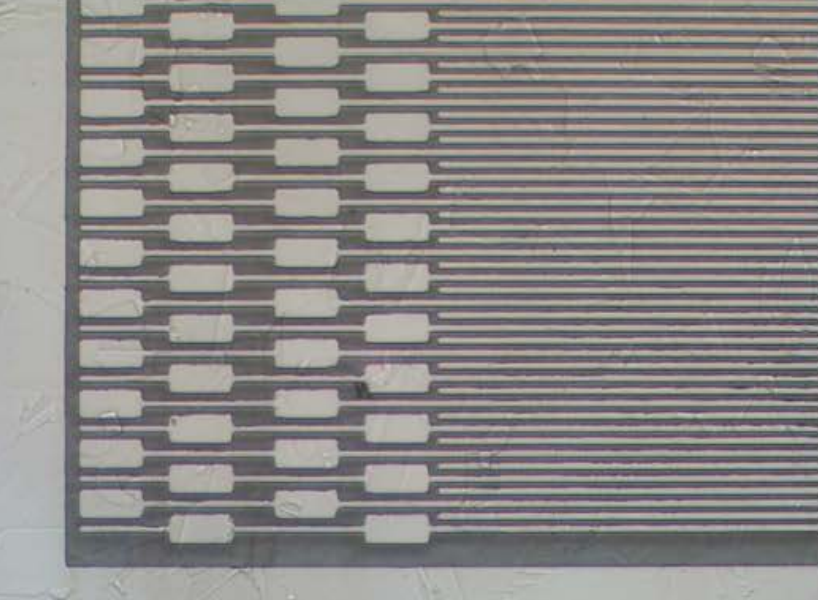
\includegraphics[height=0.4\textheight]{RadMetal}
			\caption{strip metalisation pattern}
		\end{subfigure}
		\begin{subfigure}{0.45\textwidth} 
			\centering
			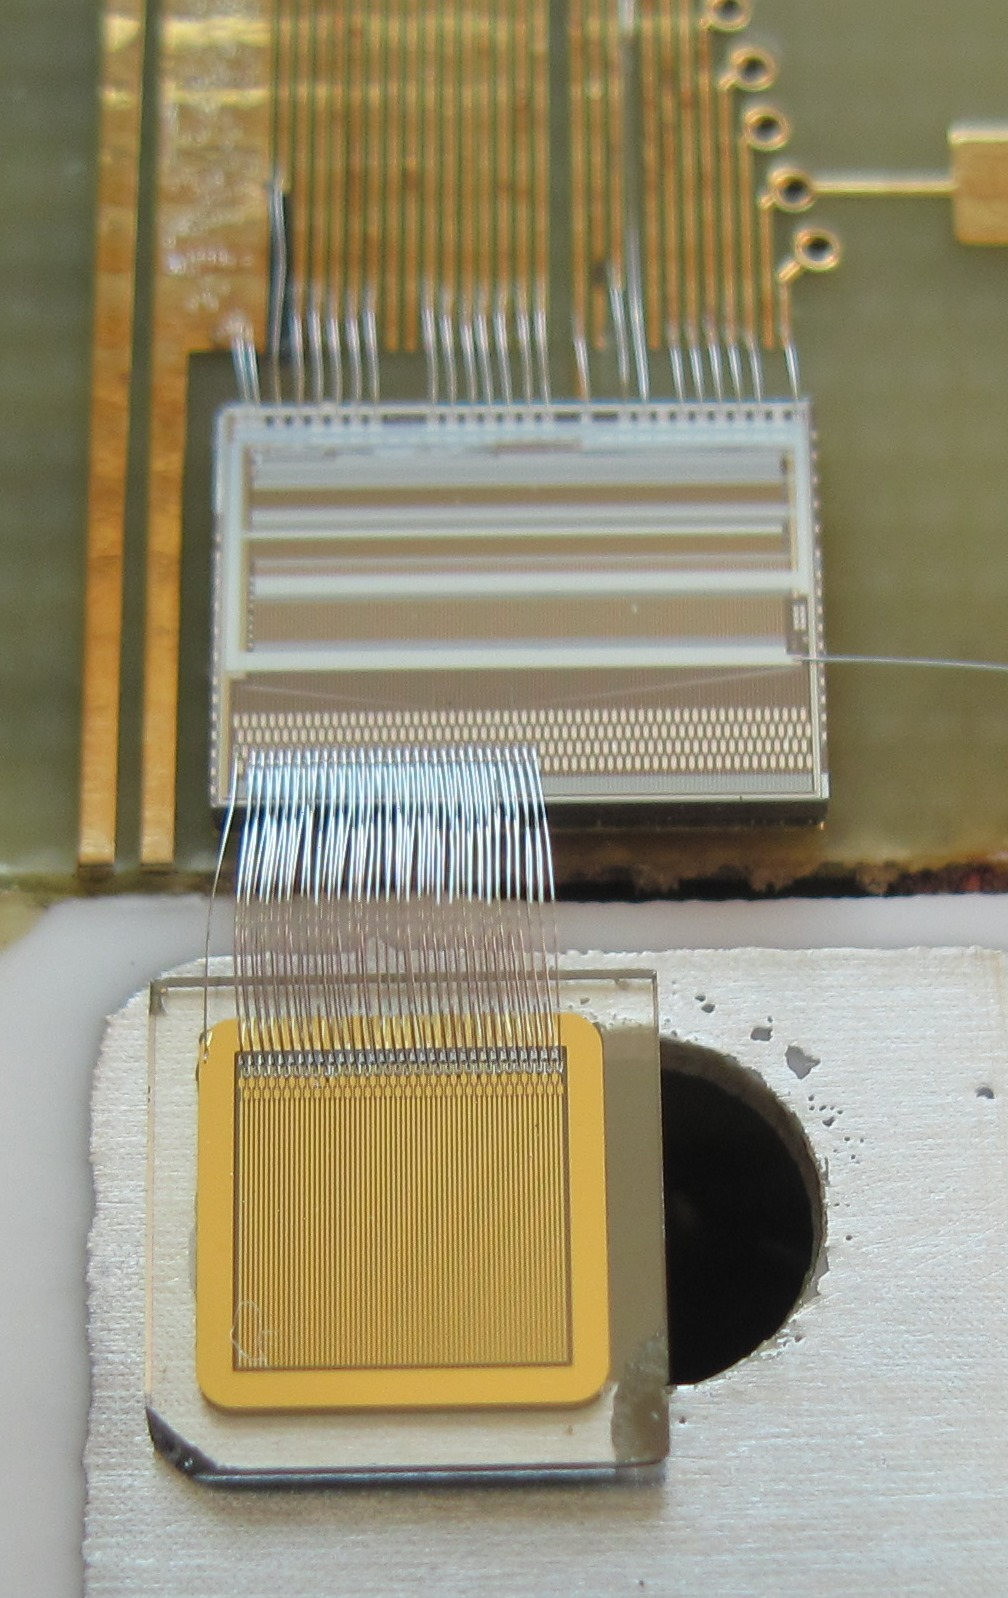
\includegraphics[width=0.4\textheight, angle=-90]{StripVA}
			\caption{mounted diamond with amplifier} 	
		\end{subfigure} 
	\end{figure}
	
	\begin{itemize}
		\itemfill
		\item patterning the diamonds \ra create pad, strip and pixel devices
		\item metalisation on both sides \ra almost edgeless 
		\item segmentation critical for radiation studies \ra charge \& position
	\end{itemize}

\end{frame}
% ============================ FRAME 2 ============================================
\begin{frame}{Schematic Beam Test Setup}

	\begin{figure}[h] 
		\centering
		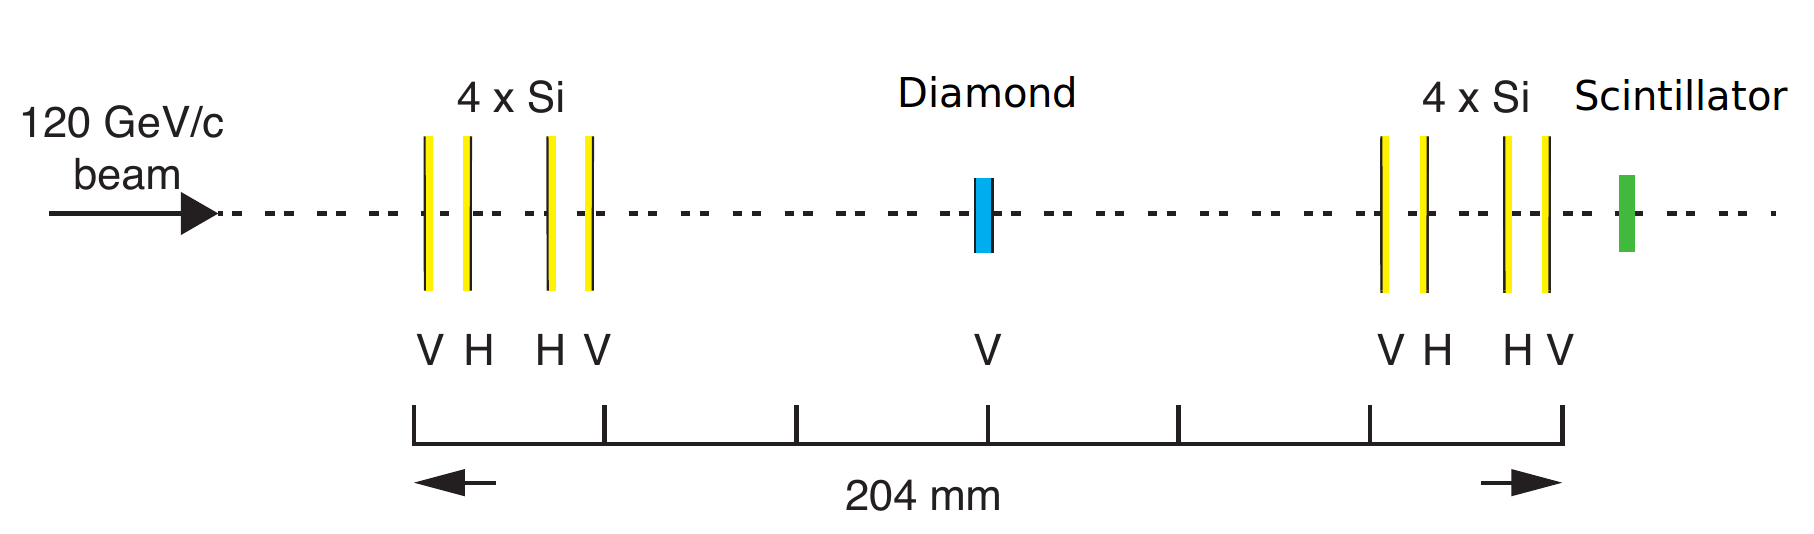
\includegraphics[width=\textwidth]{RadTel}
	\end{figure}
	
	\begin{itemize}
		\itemfill
		\item characterisation of irradiated devices in beam tests
		\item transparent or unbiased hit predictions from telescope
	\end{itemize}

\end{frame}

\subsection{Results}
% ============================ FRAME 3 ============================================
\begin{frame}{Irradiation at CERN PS with \SI{24}{\giga\electronvolt} protons}

	\begin{minipage}{4.5cm}
		\underline{damage equation:}
		\vspace*{-3pt}
		\begin{align*}
			\z{n} 				&= \z{n}_0 + \z{k}\upphi\\
			\frac{1}{\z{mfp}}	&= \frac{1}{\z{mfp}_0} + \z{k}\upphi
		\end{align*}
		\vspace*{-5pt}
		\begin{itemize}
			\item[\textcolor{black}{$\z{n}_0$}] $-$ initial number of traps
			\item[\textcolor{black}{$\z{mfp}_0$}] $-$ initial mean free path
			\item[\textcolor{black}{k}] $-$ damage constant
			\item[\textcolor{black}{$\upphi$}] $-$ fluence
		\end{itemize}
	\end{minipage}
	\hspace*{2pt}
	\begin{minipage}{6.5cm}
		\begin{figure}[h]
			\centering
			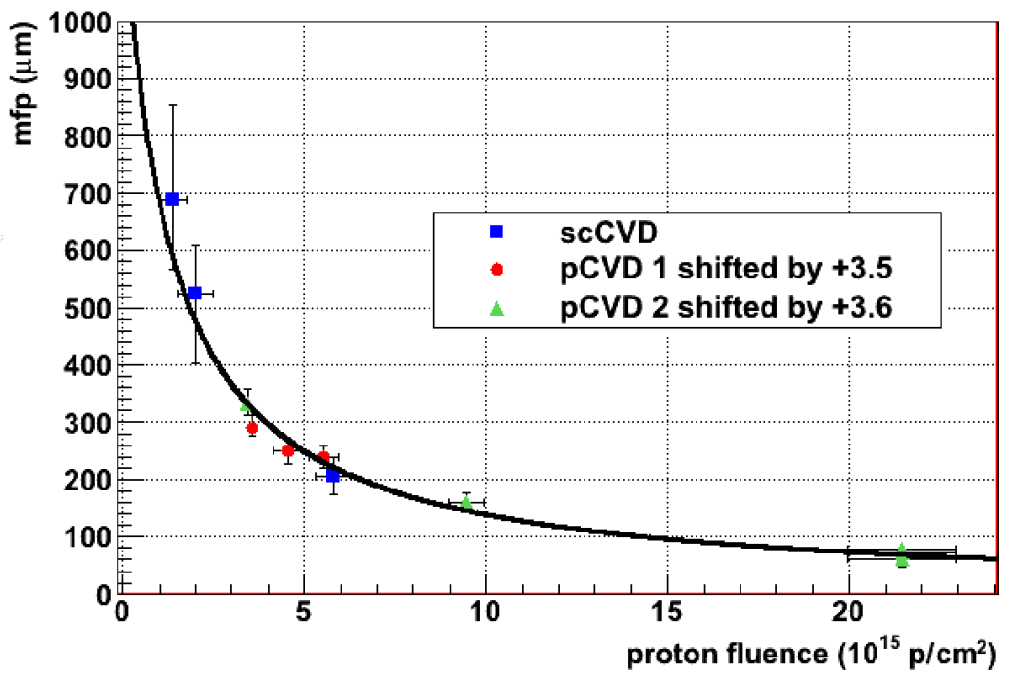
\includegraphics[width=6.5cm]{Damage24}
		\end{figure}
	\end{minipage}
	
	\begin{itemize}
		\itemfill
		\item assume same mean free path for electrons and holes
		\item results up to \SI{2.2e16}{p\per cm^2} (\SI{\sim500}{\mega rad})
		\item same damage curves and constant (k) for scCVD and pCVD diamonds
		\item larger $\z{mfp}_0$ performs better at any fluence 
	\end{itemize}

\end{frame}
% ============================ FRAME 4 ============================================
\begin{frame}{Charge Collection Distance (ccd) vs. Mean Free Path (mfp)}
	
	\begin{itemize}
		\itemfill
		\item ccd = average distance between electron and hole until trapped
		\item for scCVD: ccd $\sim$ thickness, for pCVD: ccd < thickness
% 		\item ccd coincides with mfp for mfp $\ll$ thickness
		\item ccd direct measurement (no correction)
		\item mfp correct theory \ra correct data with assumptions (i.\,a. $\z{mfp}_{\z{e}}=\z{mfp}_{\z{h}}$)
	\end{itemize}
	
	\begin{minipage}{6cm}
		\underline{equation for ccd:}
		\vspace*{-3pt}
		\begin{equation*}
			\frac{\z{ccd}}{\z{t}} = \sum_i \frac{\z{mfp}_i}{\z{t}}\left(1-\frac{\z{mfp}_i}{\z{t}}\left(1-\z{e}^{-\frac{\z{t}}{\z{mfp}_i}}\right)\right)
		\end{equation*}
		\vspace*{-5pt}
		\begin{itemize}
			\item[\textcolor{black}{t}] $-$ thickness
			\item[\textcolor{black}{$i$}] $-$ electrons \& holes
		\end{itemize}
	\end{minipage}
	\hspace*{2pt}
	\begin{minipage}{5cm}
		\begin{figure}[h]
			\centering
			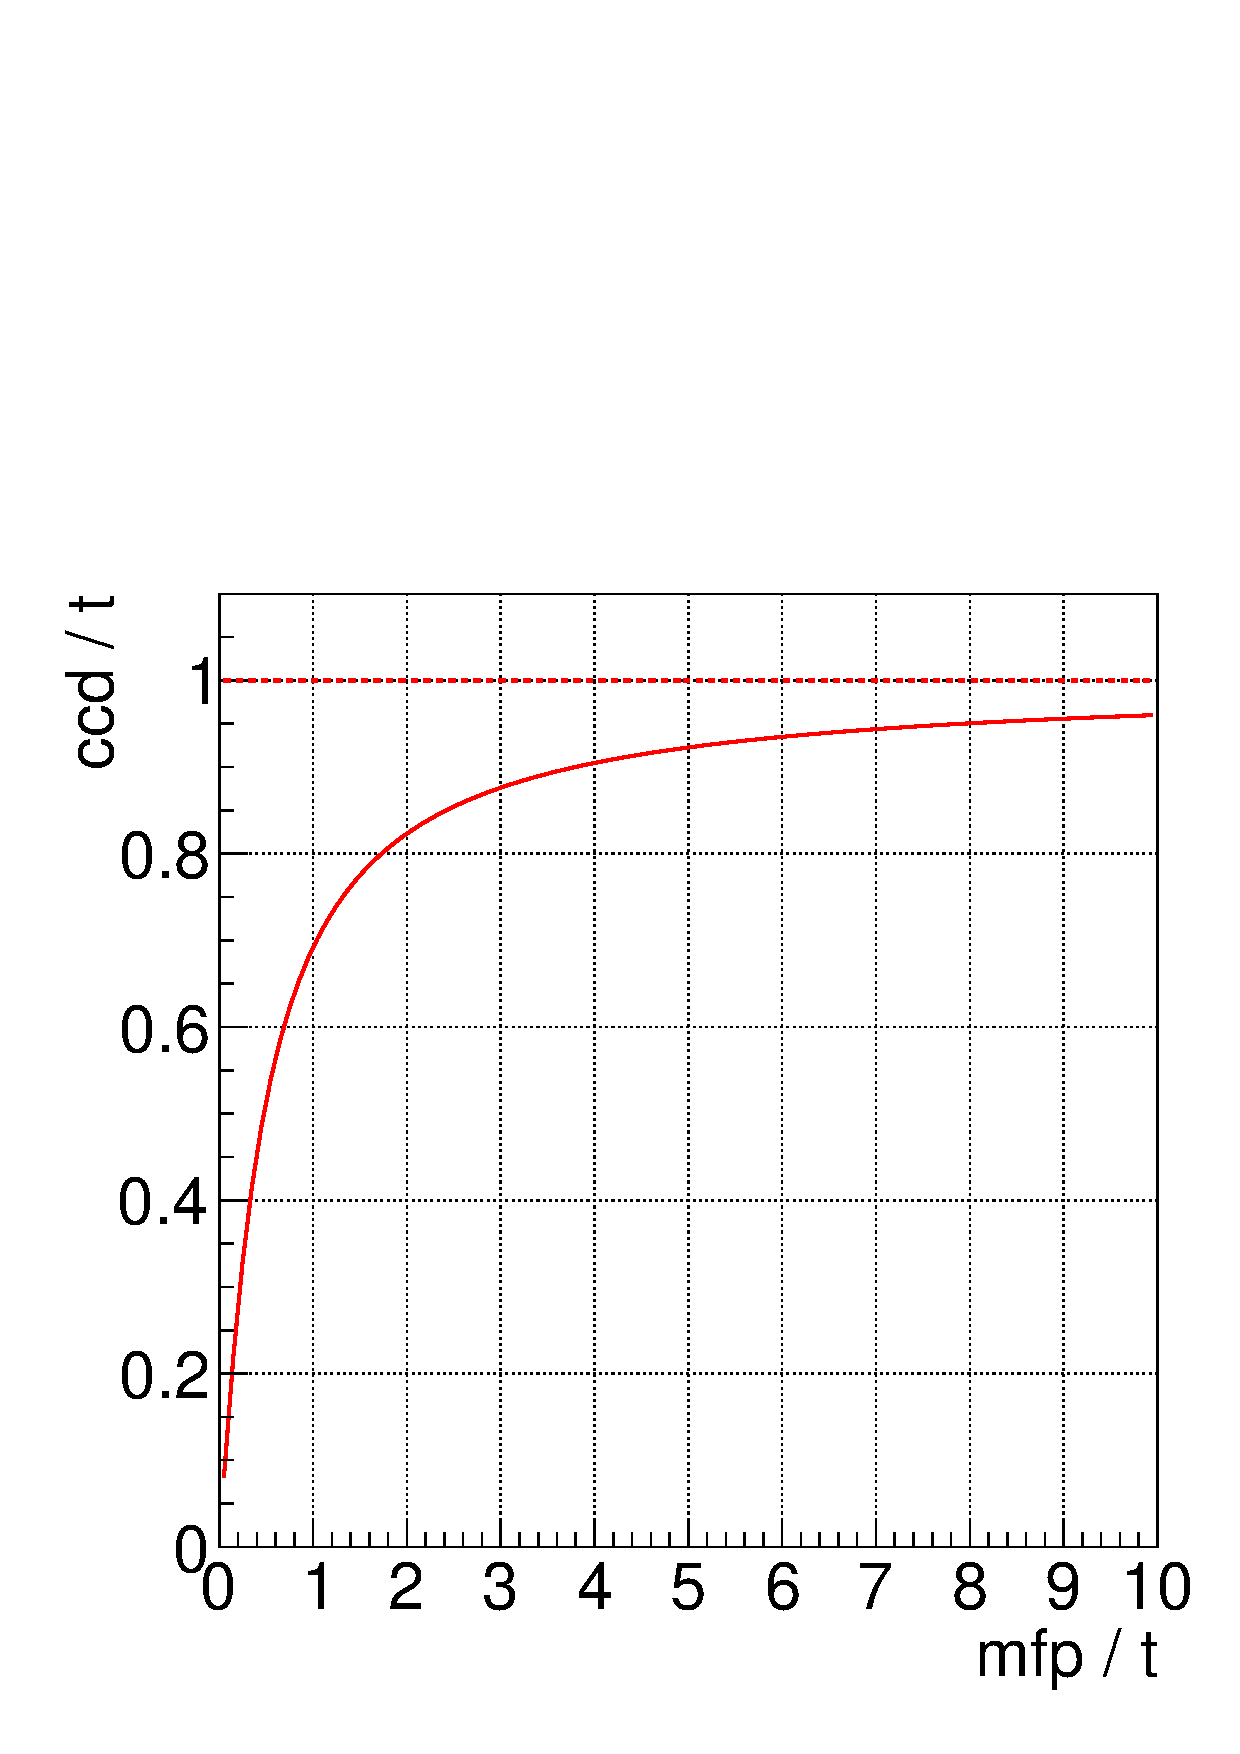
\includegraphics[width=4.5cm]{CCDMFP}
		\end{figure}
	\end{minipage}

\end{frame}
% ============================ FRAME 5 ============================================
% \begin{frame}{Irradiation at LANL with \SI{800}{\mega\electronvolt} protons}
% 
% 	\begin{figure}[h] 
% 		\centering
% 		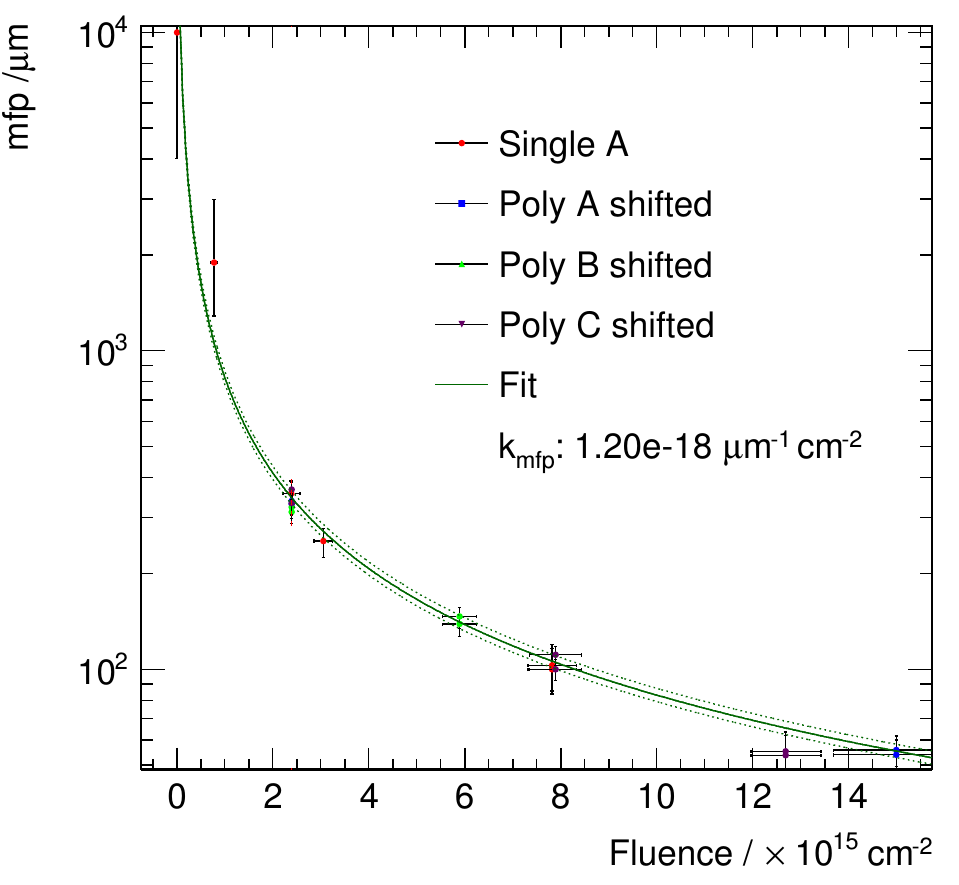
\includegraphics[width=.3\textwidth]{Damage800}
% 	\end{figure}
% 	
% 	\begin{itemize}
% 		\itemfill
% 		\item irradiation results up to \SI{1.4e16}{p\per cm^2}
% 		\item same damage curve:
% 	\end{itemize}
% 	\vspace*{-5pt}
% 	\begin{equation*}
% 		\frac{1}{\z{mfp}} = \frac{1}{\z{mfp}_0} + \z{k}\upphi
% 	\end{equation*}
% 	\vspace*{-5pt}
% 	\begin{itemize}
% 		\item \SI{800}{\mega\electronvolt} protons \SIrange{1.6}{1.8}{} more damaging than \SI{24}{\giga\electronvolt} protons
% 	\end{itemize}
% 
% \end{frame}
% ============================ FRAME 6 ============================================
\begin{frame}{Summary of Proton, Neutron and Pion Irradiation}

	\begin{figure}[h] 
		\centering
		\begin{subfigure}{0.45\textwidth}  
			\centering
			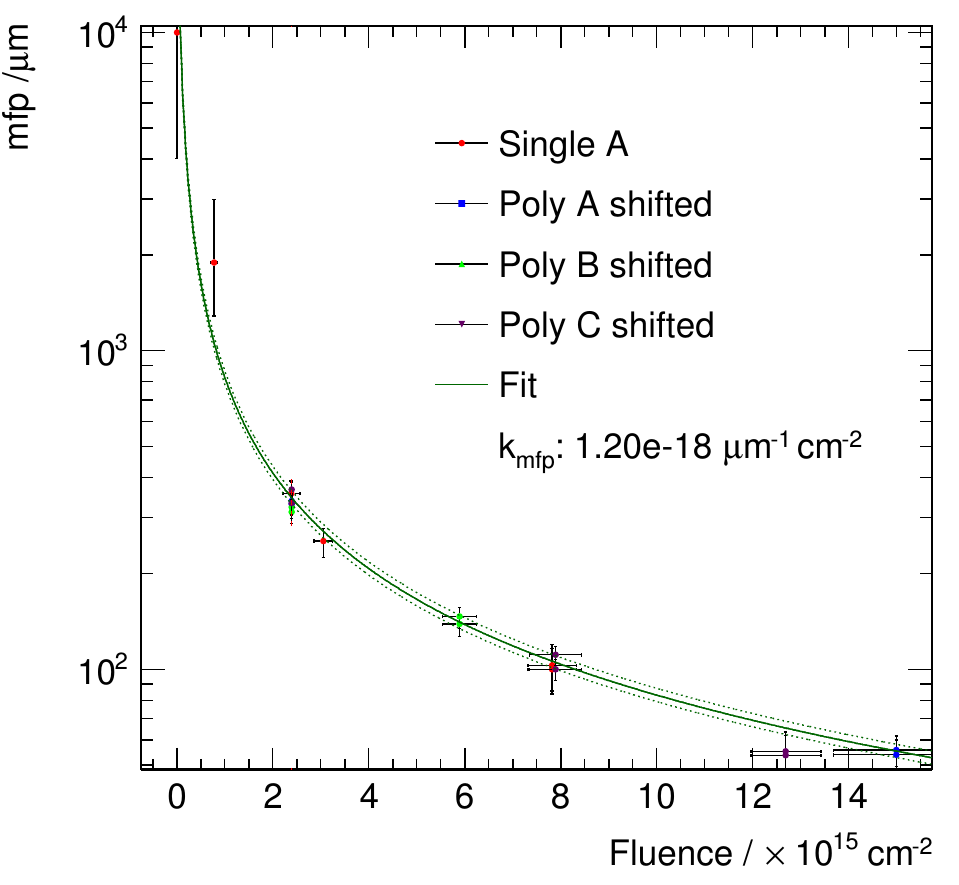
\includegraphics[height=0.5\textheight]{Damage800}
			\caption{irradiation at LANL with \SI{800}{\mega\electronvolt} protons (up to \SI{1.4e16}{p\per cm^2})}
		\end{subfigure}
		\begin{subfigure}{0.45\textwidth} 
			\centering
			\vspace*{25pt}
			\begin{tabular}[c]{l|l|l}
				\noalign{\hrule height 1pt}
				\rowcolor{title in head/foot.bg!70!white} 
	% 			\rowcolor{author in head/foot.bg} 
	% 			\rowcolor{date in head/foot.bg} 
				\multicolumn{1}{c|}{\textbf{Particle}} & \multicolumn{1}{c|}{\textbf{Energy}} & \multicolumn{1}{c}{\textbf{Relative k}} \\\hline
				\rowcolor{date in head/foot.bg!30!white} 
				Proton 	& \SI{24}{\giga\electronvolt} 	& $1.0$ 			\\\hline
						& \SI{800}{\mega\electronvolt} 	& $1.79 \pm 0.13$ 	\\\hline
				\rowcolor{date in head/foot.bg!30!white} 
						& \SI{70}{\mega\electronvolt} 	& $2.4 	\pm 0.4$ 	\\\hline
						& \SI{25}{\mega\electronvolt} 	& $4.5 	\pm 0.6$ 	\\\hline
				\rowcolor{date in head/foot.bg!30!white} 
				Neutron	& \SI{1}{\mega\electronvolt} 	& $4.5 	\pm 0.5$ 	\\\hline
				Pion	& \SI{200}{\mega\electronvolt} 	& $2.5 	- 3$ 		\\
				\noalign{\hrule height 1pt}
			\end{tabular}
			\caption{summary}
		\end{subfigure}
	\end{figure}
	
% 	\begin{itemize}
% 		\item data fits displacement energy (DPA) better than non ionising energy loss (NIEL) theories
% 		\item DPA need to be tuned to diamonds
% 	\end{itemize}

\end{frame}
